\documentclass[a4paper]{article}
\usepackage{setspace}
\usepackage[T2A]{fontenc} %
\usepackage[utf8]{inputenc} % подключение русского языка
\usepackage[russian]{babel} %
\usepackage[12pt]{extsizes}
\usepackage{mathtools}
\usepackage{graphicx}
\usepackage{fancyhdr}
\usepackage{amssymb}
\usepackage{amsmath, amsfonts, amssymb, amsthm, mathtools}
\usepackage{tikz}

\usetikzlibrary{positioning}
\setstretch{1.3}

\newcommand{\mat}[1]{\begin{pmatrix} #1 \end{pmatrix}}
\renewcommand{\det}[1]{\begin{vmatrix} #1 \end{vmatrix}}
\renewcommand{\f}[2]{\frac{#1}{#2}}
\newcommand{\dspace}{\space\space}
\newcommand{\s}[2]{\sum\limits_{#1}^{#2}}
\newcommand{\mul}[2]{\prod_{#1}^{#2}}
\newcommand{\sq}[1]{\left[ {#1} \right]}
\newcommand{\gath}[1]{\left[ \begin{array}{@{}l@{}} #1 \end{array} \right.}
\newcommand{\case}[1]{\begin{cases} #1 \end{cases}}
\newcommand{\ts}{\text{\space}}
\newcommand{\lm}[1]{\underset{#1}{\lim}}
\newcommand{\suplm}[1]{\underset{#1}{\overline{\lim}}}
\newcommand{\inflm}[1]{\underset{#1}{\underline{\lim}}}

\renewcommand{\phi}{\varphi}
\newcommand{\lr}{\Leftrightarrow}
\renewcommand{\r}{\Rightarrow}
\newcommand{\rr}{\rightarrow}
\renewcommand{\geq}{\geqslant}
\renewcommand{\leq}{\leqslant}
\newcommand{\RR}{\mathbb{R}}
\newcommand{\CC}{\mathbb{C}}
\newcommand{\QQ}{\mathbb{Q}}
\newcommand{\ZZ}{\mathbb{Z}}
\newcommand{\VV}{\mathbb{V}}
\newcommand{\NN}{\mathbb{N}}

\DeclarePairedDelimiter\abs{\lvert}{\rvert} %
\makeatletter                               % \abs{}
\let\oldabs\abs                             %
\def\abs{\@ifstar{\oldabs}{\oldabs*}}       %

\begin{document}

\section*{Домашнее задание на 13.11 (Линейная алгебра)}
 {\large Емельянов Владимир, ПМИ гр №247}\\\\
\begin{enumerate}
    \item[\textbf{1.}]$\mat{A & B \\ 0 & C}\cdot \mat{A_1 & B_1 \\ C_1 & D_1} = \mat{E & 0 \\ 0 & E}$, $A_1, B_1, C_1, D_1?$
    $$\mat{A & B \\ 0 & C}\cdot \mat{A_1 & B_1 \\ C_1 & D_1} = \mat{AA_1 +BC_1 & AB_1+BD_1 \\ CC_1 & CD_1} = \mat{E & 0 \\ 0 & E} \r$$
    $$\r \case{
        AA_1 +BC_1 = E \\
        AB_1+BD_1 = 0 \\
        CC_1 =0 \r C_1 = 0\\
        CD_1 = E \r D_1 = C^{-1}E 
    }\r \case{
        AA_1 = E \\
        AB_1+BC^{-1} = 0 \\
        C_1 = 0\\
        D_1 = C^{-1}
    }\r \case{
        A_1 = A^{-1} \\
        B_1= -A^{-1}BC^{-1} \\
        C_1 = 0\\
        D_1 = C^{-1}
    } \r $$
    $$\r \mat{A_1 & B_1 \\ C_1 & D_1} = \mat{A^{-1}  & -A^{-1}BC^{-1} \\ 0 & C^{-1}}$$
    \textbf{Ответ: }$\mat{A^{-1}  & -A^{-1}BC^{-1} \\ 0 & C^{-1}}$\\

    \item[\textbf{2.}]$\f{(5+i)(7-6i)}{3+i}$
    $$\f{(5+i)(7-6i)}{3+i} = \f{35+7i-30i-6i^2}{3+i} = \f{35-23i+6}{3+i} = \f{41-23i}{3+i} = \f{(41-23i)(3-i)}{9+1} =$$
    $$= \f{123-69i-41i-23}{10} =  \f{100-110i}{10} = 10 - 11i$$
    \textbf{Ответ: }$10 -11i$\\

    \item[\textbf{3.}]
    \begin{enumerate}
        \item[1)]$$\det{a + bi & c + di \\ -c +di & a-bi} = (a + bi)(a-bi) - (c + di)(-c +di) = a^2 + b^2 - (-d^2-c^2) = $$
        $$ = a^2 + b^2 +d^2+c^2$$
        \item[2)]$$\det{\cos \alpha + i \sin \alpha & 1 \\ 1 & \cos \alpha - i \sin \alpha} = (\cos \alpha + i \sin \alpha)(\cos \alpha - i \sin \alpha) - 1 = $$
        $$=\cos^2 \alpha + \sin^2 \alpha - 1 = 1- 1 = 0$$
        \item[3)]$$\det{1 & 0 & 1 + i \\ 0 & 1 & i \\ 1-i & -i & 1} = \det{1 & 0 & 1 + i \\ 0 & 1 & i \\ 0 & -i & 1-(1-i^2)} = \det{1 & 0 & 1 + i \\ 0 & 1 & i \\ 0 & -i & -1}= \det{1 & 0 & 1 + i \\ 0 & 1 & i \\ 0 & 0 & i^2-1} =$$
        $$=\det{1 & 0 & 1 + i \\ 0 & 1 & i \\ 0 & 0 & -2} = -2$$
    \end{enumerate}

    \item[\textbf{4.}]
    $$\case{
        (1+i)z_1 + (1-i)z_2 = 1 + i \\
        (1-i)z_1 + (1+i)z_2 = 1 + 3i
    }$$
    Запишем в виде матрицы СЛУ:
    $$A = \mat{1+i & 1-i &| &1 + i \\ 1-i & 1+i & | & 1 + 3i} $$
    $$A_{(1)} = A_{(1)} + A_{(2)} \to \mat{2 & 2 &| & 2+4i \\ 1-i & 1+i & | & 1 + 3i}$$
    $$A_{(1)} = A_{(1)}/2 \to \mat{1 & 1 &| & 1+2i \\ 1-i & 1+i & | & 1 + 3i}$$
    $$A_{(2)} = A_{(2)}-A_{(1)}*(1-i) \to \mat{1 & 1 &| & 1+2i \\ 0 & 2i & | & -2 + 2i}$$
    $$A_{(2)} = A_{(2)}/(2i) \to \mat{1 & 1 &| & 1+2i \\ 0 & 1 & | & 1+i}$$
    $$A_{(1)} = A_{(1)}-A_{(2)} \to \mat{1 & 0 &| & i \\ 0 & 1 & | & 1+i}$$
    \textbf{Ответ: } $\case{z_1 = i \\ z_2 = 1+i}$\\

    \item[\textbf{5.}]$$A = \mat{1+i & 1-i  \\ 1-i & 1+i} \r det A = (1+i)^2-(1-i)^2 = 4i$$
    $$A_{z_1} = \mat{1 + i & 1-i  \\ 1 + 3i & 1+i} \r detA_{z_1} = (1+i)^2-(1-i)(1+3i) = -4$$
    $$A_{z_2} = \mat{1+i & 1 + i  \\ 1-i & 1 + 3i} \r detA_{z_2} = (1+i)(1+3i)-(1-i^2) = -4 + 4i$$
    $$z_1 = \f{detA_{z_1}}{detA} = \f{-4}{4i}=-\f{1}{i} = -\f{i}{-1} = i$$
    $$z_2 = \f{detA_{z_2}}{detA} = \f{-4+4i}{4i} = -\f{1}{i} + 1 = i+1$$
    \textbf{Ответ: } $\case{z_1 = i \\ z_2 = 1+i}$\\

    \item[\textbf{6.}]
    \begin{enumerate}
        \item[1)]    $$-3i = 3(0-i) = 3(\cos{(-\f{\pi}{2})} + i\sin{(-\f{\pi}{2})})$$
        \item[2)]    $$1+\f{\sqrt{3}}{3}i = \f{2}{\sqrt{3}}(\f{\sqrt{3}}{2} + \f{1}{2}i) = \f{2}{\sqrt{3}}(\cos{\f{\pi}{6}}+i\sin{\f{\pi}{6}})$$
        \item[3)]    $$\f{\cos \phi + i \sin \phi}{\cos \psi + i \sin \psi} = \cos (\phi - \psi) + i \sin (\phi - \psi)$$\\
    \end{enumerate}

    \item[\textbf{7.}]$(\sqrt{3}-i)^{32}$
    $$(\sqrt{3}-i)^{32} = (2(\f{\sqrt{3}}{2}-\f{1}{2}i))^{32} = (2(\cos \f{\pi}{6}-i\sin\f{\pi}{6}))^{32} = 2^{32}(\cos \f{32\pi}{6}-i\sin\f{32\pi}{6}) = $$
    $$=2^{32}(\cos(5\pi + \f{\pi}{3})-i\sin(5\pi + \f{\pi}{3})) = -2^{32}(\cos(\f{\pi}{3})-i\sin(\f{\pi}{3})) = $$
    $$= -2^{32}(\f{1}{2}-i\f{\sqrt{3}}{2}) = -2^{31}+i2^{31}\sqrt{3}$$
    \textbf{Ответ: } $-2^{32}(\cos(\f{\pi}{3})-i\sin(\f{\pi}{3})) \;$ и $ \; -2^{31}+i2^{31}\sqrt{3}$\\

    \item[\textbf{8.}]
    \begin{enumerate}
        \item[$z_1$]
        $$z_1^3 = 2-2i = 2\sqrt{2}(\f{1}{\sqrt{2}} - \f{1}{\sqrt{2}}i) = 2\sqrt{2}(\cos{(\f{\pi}{4} + 2\pi k)} - i\sin{(\f{\pi}{4} + 2\pi k)}), k \in \ZZ \r $$
        $$\r z_1 = \sqrt[3]{2\sqrt{2}}(\cos{(\f{\pi}{12}+\f{2\pi k}{3})} - i\sin{(\f{\pi}{12}+\f{2\pi k}{3})}) = $$
        $$=\sqrt{2}(\cos{(\f{\pi}{12}+\f{2\pi k}{3})} - i\sin{(\f{\pi}{12}+\f{2\pi k}{3})}), k = 0, 1, 2$$
        \[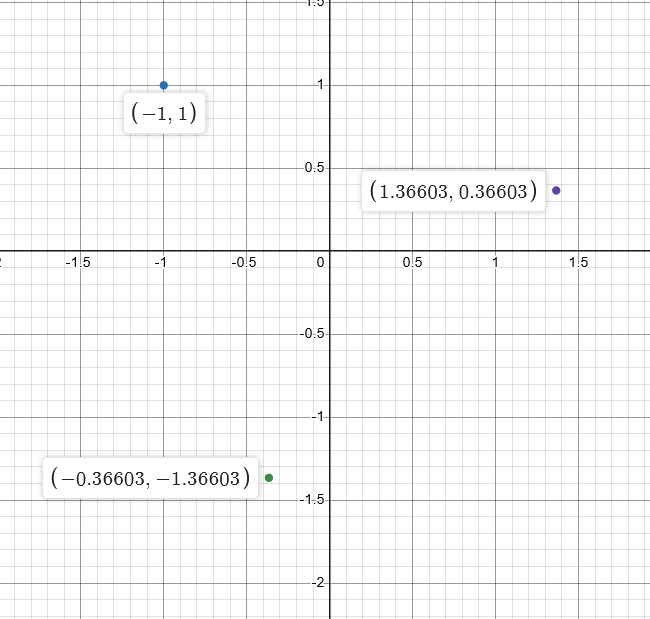
\includegraphics[width=0.8\textwidth]{image1.png}\]
        \item[$z_2$]
        $$z_2^6 = (2-2i)^2 = 4-8i-4 = -8i = 8(0-i) = 8(\cos (\f{\pi}{2} + 2\pi n) -i \sin (\f{\pi}{2} + 2\pi n)), n \in Z \r$$
        $$\r z_2 = \sqrt[6]{2^3}(\cos (\f{\pi}{12} + \f{\pi n}{3}) -i \sin (\f{\pi}{12} + \f{\pi n}{3})) =$$
        $$= \sqrt{2}(\cos (\f{\pi}{12} + \f{\pi n}{3}) -i \sin (\f{\pi}{12} + \f{\pi n}{3})), n=0,1,2,3,4,5$$
        \[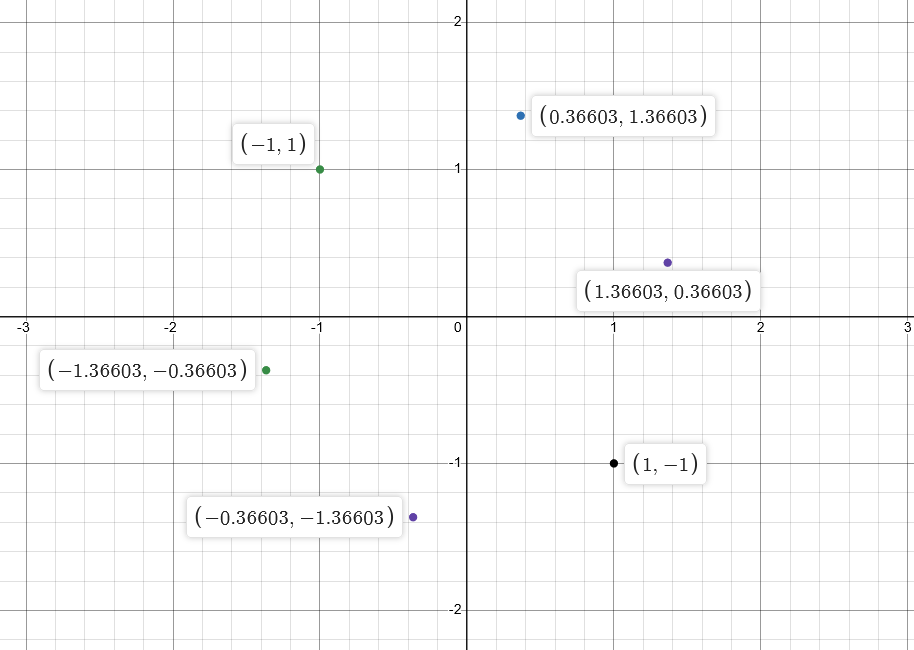
\includegraphics[width=0.9\textwidth]{image2.png}\]\\
    \end{enumerate}

    \item[\textbf{9.}]$\sqrt[4]{\f{-18}{1+i\sqrt{3}}} = z$
    $$z^4 = \f{-18}{1+i\sqrt{3}} = \f{-18(1-i\sqrt{3})}{4} = \f{-18+18i\sqrt{3}}{4} = \f{-9+9i\sqrt{3}}{2} = 9(-\f{1}{2} + i\f{\sqrt{3}}{2}) = $$
    $$ = 9(cos(\f{2 \pi}{3} + 2\pi k)+i \sin(\f{2 \pi}{3} + 2\pi k)), k \in \ZZ$$
    $$z = \sqrt{3}(cos(\f{\pi}{6} + \f{\pi k}{2})+i \sin(\f{\pi}{6} + \f{\pi k}{2})), k =0,1,2,3$$
    $$\case{
        k = 0: z = \sqrt{3}(cos(\f{\pi}{6})+i \sin(\f{\pi}{6})) = \f{3}{2}+i\f{\sqrt{3}}{2}\\
        k = 1: z = \sqrt{3}(cos(\f{\pi}{6} + \f{\pi}{2})+i \sin(\f{\pi}{6} + \f{\pi}{2})) = -\f{\sqrt{3}}{2}+i\f{3}{2}\\
        k = 2: z = \sqrt{3}(cos(\f{\pi}{6} + \pi)+i \sin(\f{\pi}{6} + \pi)) = -\f{3}{2}-i\f{\sqrt{3}}{2}\\
        k = 3: z = \sqrt{3}(cos(\f{\pi}{6} + \f{3\pi}{2})+i \sin(\f{\pi}{6} + \f{3\pi}{2})) = \f{\sqrt{3}}{2} - i \f{3}{2} \\
    }$$
    \[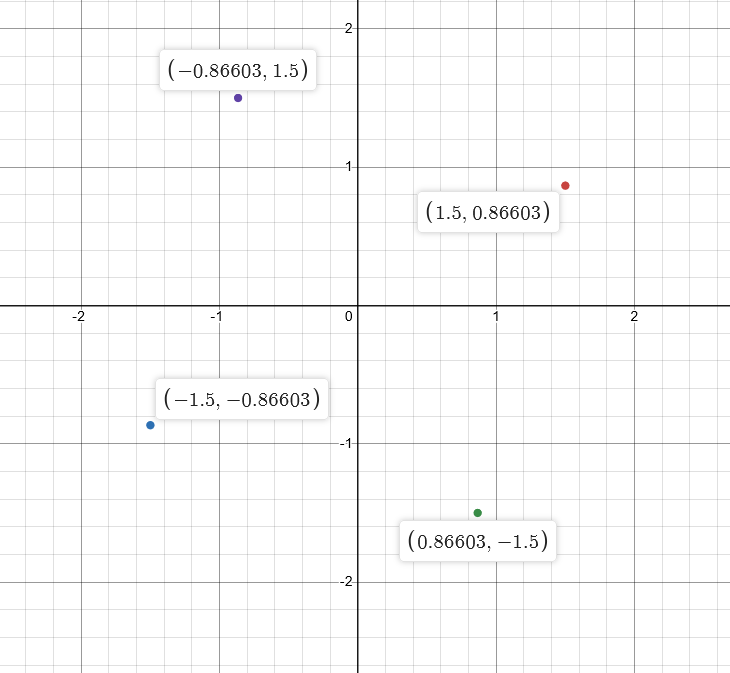
\includegraphics[width=0.9\textwidth]{image3.png}\]\\

    \item[\textbf{10}]$(2\sqrt{3}-i)z^4 = 10-6\sqrt{3}i$
    \begin{enumerate}
        \item[1)] $(2\sqrt{3}-i) = 0:$
        $$0 = 10-6\sqrt{3}i \; \; \varnothing$$

        \item[2)]$(2\sqrt{3}-i) \neq 0:$
        $$z^4 = \f{10-6\sqrt{3}i}{2\sqrt{3}-i}=\f{(10-6\sqrt{3}i)(2\sqrt{3}+i)}{13} = \f{26\sqrt{3} - 26i}{13} = 2\sqrt{3}-2i = $$
        $$ = 4(\f{\sqrt{3}}{2}-i\f{1}{2}) = 4(\cos(\f{\pi}{6} + 2\pi k)-i\sin{(\f{\pi}{6} + 2\pi k)}), k \in \ZZ \r$$
        $$\r z = \sqrt{2}(\cos(\f{\pi}{24} + \f{\pi k}{2})-i\sin(\f{\pi}{24} + \f{\pi k}{2}))$$
        Найдём $k$ при которых аргумент решения принадлежит $(\f{5\pi}{2}, 3\pi)$:
        $$\f{5\pi}{2}< \f{\pi}{24} + \f{\pi k}{2} < 3\pi$$
        $$\f{5\pi}{2}-\f{\pi}{24}< \f{\pi k}{2} < 3\pi-\f{\pi}{24}$$
        $$\f{59\pi}{24}<\f{\pi k}{2} < \f{71\pi}{24}$$
        $$\f{59}{12}<k< \f{71}{12}$$
        $$4\f{11}{12}<k< 5\f{11}{12} \r k = 5, \text{ т.к. } k \in \ZZ$$
        $$k = 5: z = \sqrt{2}(\cos(\f{\pi}{24} + \f{5\pi}{2})-i\sin(\f{\pi}{24} + \f{5\pi}{2})) = \sqrt{2}(\cos(\f{61\pi}{24})-i\sin(\f{61\pi}{24}))$$
        \textbf{Ответ: } $\sqrt{2}(\cos(\f{61\pi}{24})-i\sin(\f{61\pi}{24}))$
    \end{enumerate}

    \item[\textbf{11}]$$(1+i)^n = \s{k=0}{n}\binom{n}{k}i^k = \binom{n}{0} + \binom{n}{1}i - \binom{n}{2} - \binom{n}{3}i+ \dots$$
    $$i\s{k=1}{[\f{n}{2}]}(-1)^{k-1}\binom{n}{2k-1} = \binom{n}{1}i - \binom{n}{3}i+\binom{n}{5}i$$
    $$C_n^0 - C_n^2$$
\end{enumerate}
\end{document}